\chapter{Phase de développement~: conception et implémentation d'un module
statistique}
	\paragraph{}
	Dans la partie précédente nous avons proposé une solution fonctionnelle aux
	besoins exprimés par les utilisateurs. Ici, nous allons concevoir la solution
	technique à partir des fonctionnalités, puis l'implémenter c'est-à-dire en
	écrire le code.
	La partie A présentera l'architecture actuelle de TrackCIS. La partie B
	présentra la conception de la solution technique. Enfin, la partie C présentera
	la méthodologie d'implémentation de cette solution. Enfin, dans la partie D, nous ferons le
	bilan de ce qui a effectivement pus être implémenté au cours de ce projet et
	nous discuterons des limites et des biais de la méthodologie ainsi que des
	suites possibles pour Xperis.
	
	\section{TrackCIS, une application web en deux parties}
		
		\subsection{Qu'est-ce qu'une application web ?}
			\paragraph{}% Modèle client serveur classique
			TrackCIS est une application accessible depuis un navigateur internet, il
			s'agit d'une application web. CLassiquement, le fonctionnement de ce type
			d'application est basé sur le modèle dit <<client-serveur>>. Un client
			correspond au navigateur internet de l'utilisateur (Chrome, FireFox\ldots),
			il permet de communiquer avec le serveur. Ce dernier est une machine sur
			laquelle est déployée l'application web. Le client envoie une requête au
			serveur qui va la traiter et générer en retour une page web au format HTML
			(Hypertext Markup Language) qui est renvoyée au client puis affichée
			(figure \ref{client_serveur}). La requête utilise le protocole HTTP
			(Hyperttext transfert protocole) qui est le protocole standard des échanges
			sur le net. La page HTML contient toues les inforamtions permettant au
			navigateur d'afficher la page. Cette page peut faire appel à d'autres
			ressources comme des pages CSS (Cascading style sheets) ou des script
			Javascript. CSS est un langage descriptif permettant de mettre en forme le contenu de la page HTML.
			Javascript est également un langage qui est interprété par le client et qui
			permet de gérer les léments dynamiques de la page web (annimations, gestion
			des évennements lorsque l'utilisateur clic sur un bouton\ldots).
			\begin{figure}[H]
				\centering
				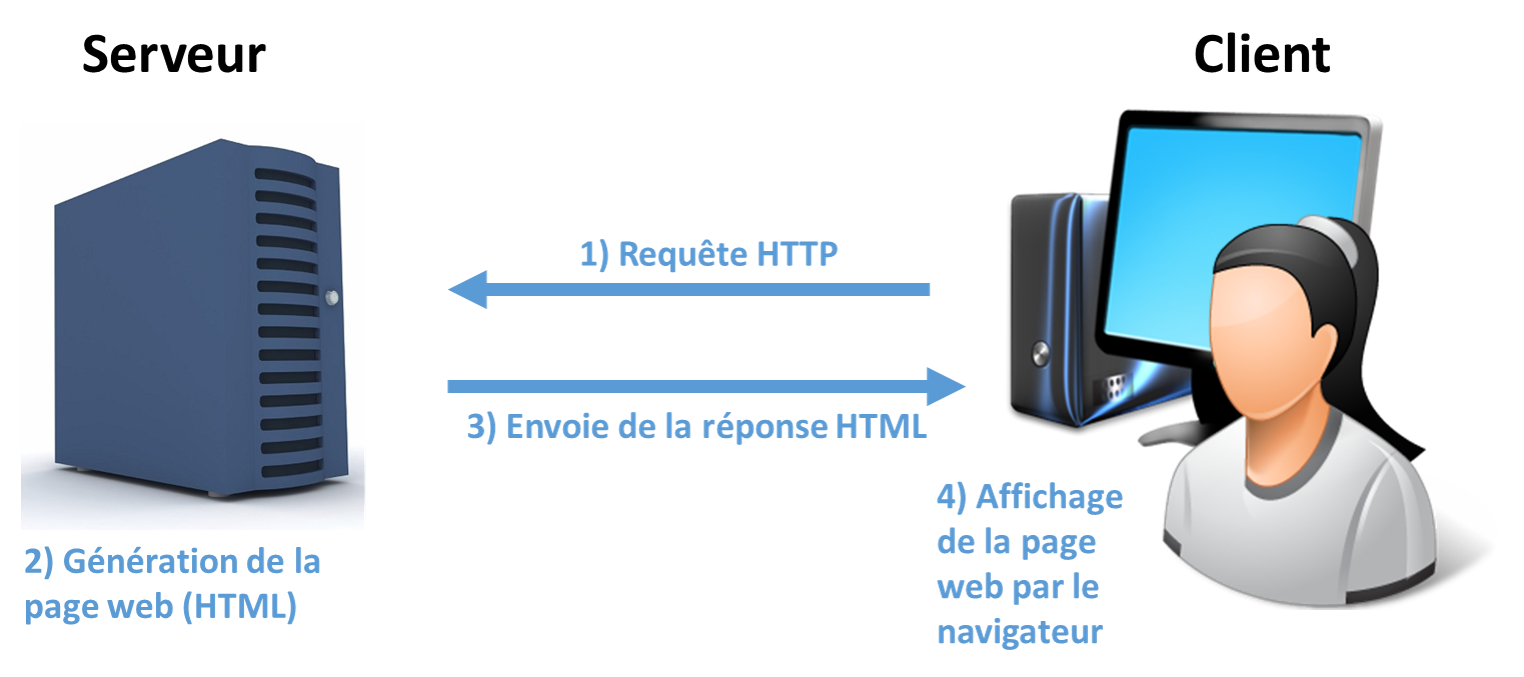
\includegraphics[width=10cm]{../img/part3/client_serveur.png}
				\caption{\label{client_serveur} Le serveur génère dynamiquement la page
				HTML qui sera affichée sur le poste client.}
			\end{figure}
			
			\paragraph{}% Modèle AJAX
			Une variante du modèle client-serveur permet d'en augmenté la rapidité, il
			s'agit du modèle AJAX (Asynchronous Javascript and XML).
			Dans le modèle précédent, toute la page doit être renvoyée par le
			serveur à chaque requête, ce qui n'est pas forcément utile. Cela pose deux
			problèmes :
			d'une part beaucoup de données transitent entre le client et le serveur,
			d'autre part le rechargement complet de la page prend du temps ce qui nuit à
			l'expérience de l'utilisateur.
			Le modèle AJAX, sur lequelle repose TrackCIS, consiste à ne recharger que les
			parties de la page qui sont concernées par la modification sans toucher aux
			autres.
			Par exemple, dans le cas de l'affichage de la liste des messages entre une
			date de début et une date de fin, si l'utilisateur modifie la période, seule
			la liste des messages sera rechargée. Le reste de la page (menu, pieds de
			page, entête\ldots) ne sera pas renvoyé par le serveur. Les appels AJAX sont
			réalisés au niveau des scripts Javascript, donc côté client.
			
		\subsection{TrackCIS est composé d'un frontal et d'une API}
			\paragraph{}% Archi générale de l'application
			TrackCIS sur les modèles client-serveur et AJAX. Les deux
			premiers éléments de l'architecture sont le client (le navigateur internet
			de l'utilisateur) et le serveur hébergant l'application web stricto-sensu,
			que nous appelerons dans la suit le <<Frontal>> (figure
			\ref{archi_trackcis}).
			Celui-ci reçoit et traite les requêtes du client. Le Frontal ne communique pas directement avec
			CLoverleaf, c'est une autre partie de l'architecture qui s'en charge : l'API.
			API sigifi Interface de propgrammation applicatve. C'est un intermédiaire
			entre deux applications. En l'occurence, l'API est l'intermédiaire entre le
			Frontal, qui a pour but d'afficher une page web, et Cloverleaf. Prenons un
			exemple : le client envoie une requête au Frontal pour afficher la liste de
			tous les messages passé sur un flux donné durant une période donnée. Le
			Frontal reçoi la requête et envoie à son tour une autre requête à l'API.
			Cette dernière récupère les informations demandées auprès de CLoverleaf et
			les transmet au Frontal. Enfin, celui-ci génère la page HTML avec la liste
			des messages et la renvoie au client.\newline
			API et Frontal sont deux entitées séparées, toutes deux développées par
			Xperis. Ils ne sont généralement pas déployés sur le même serveur. L'API est
			nécessairement installée sur le même serveur que CLoverleaf, le Frontal est
			lui généralement installé sur un serveur à part situé au
			sein de l'établissement hospitalier d'un serveur.
			\begin{figure}[H]% Architecture globale de l'application
				\centering
				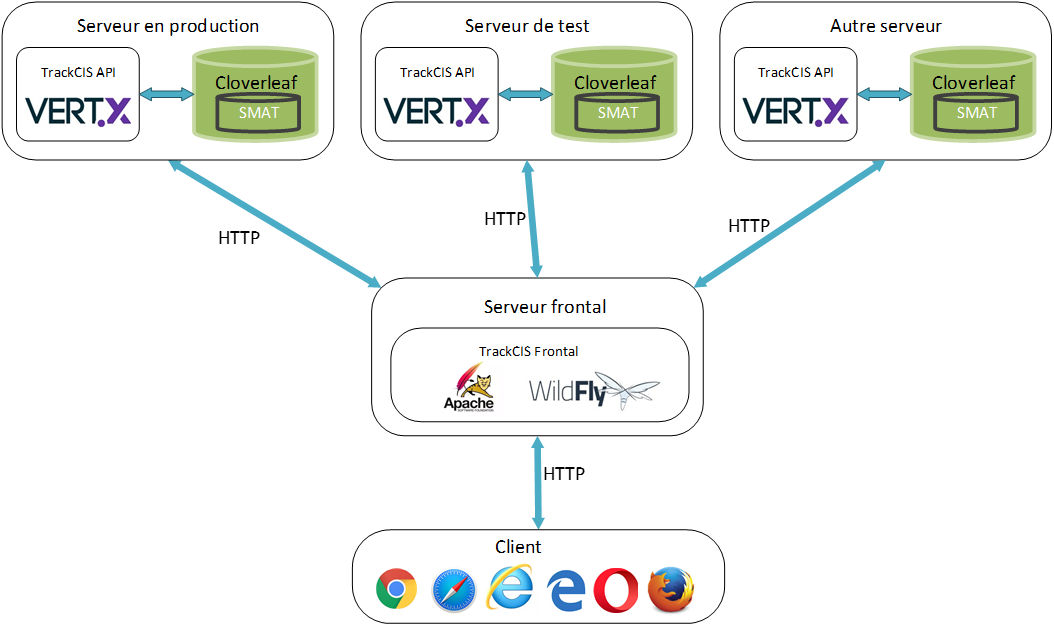
\includegraphics[width=10cm]{../img/part3/archi_trackcis.png}
				\caption{\label{archi_trackcis} TrackCIS est composés de deux éléments
				distincts pouvant se trouver sur deux serveurs différents.}
			\end{figure}
			Frontal et API sont tous deux développés avec le langage Java.
			
		\subsection{Le frontal est développé en java J2EE}
			\paragraph{}% les grandes lignes de l'archi du front
			Java Entreprise Edition, que nous désignerons par J2EE, est une
			plateforme basée sur le langage Java et destinée au développement web. Il
			s'agit d'un ensemble de bibliothèques Java mettant à dispostion des
			développeurs les éléments nécessaire au développement d'une application
			web.
			
			\paragraph{}
			Java à la particularité d'être un langage orienté objet. Le code est organisé
			en classes. Chaque classe peut possèder un certain nombre d'attributs
			(données stockées sous la forme de variables) et de méthodes (opérations
			que la classe est capable d'effectuer).La figure \ref{archi_actuelle_front}
			résume l'architecture actuelle du Frontla de TrackCIS. Chaque bloc représente
			un groupe de classes ayant des rôles similaires. Globalement, le Frontal
			respecte l'architecture dite MVC (Modèle, contrôle, vue) qui permet de
			diviser le code en trois grand rôle : les traitements (Modèle) la génération
			de la page HTML (la Vue) et des classes faisant office d'intermédiaire entre
			Modèle et Vue (les Contrpoleur). (1) La requête HTTP envoyée par le client et
			reçue au niveau des classes dites <<contrôleur>>. Ces classes en font appel
			à d'autres : les classes de service. Celle-ci effectuent les oppérations les
			plus complexes (2). Les classes de répertoire (ou repositories) communiquent
			avec la base de donnée (3). Cette dernière permet de stocker les préférences
			des utilsateurs ainsi que d'autres données permettant de se connecter à
			l'API (adresse du serveur de CLoverleaf, port utilisé\ldots). Les classes de
			répertoire permettent d'envoyer des requêtes SQL à cette base de données
			pour en lire les informations ou les mettre à jour. Lss classes de données
			(4) contiennent essentiellement des attribue et mais peu de méthodes. Comme
			leur nom l'indique elles permettent de stocker des données : les données
			récupéreées par les répertoires depuis la base de donnée, ou bien les
			données renvoyées par l'API (6). Certaines classes de services (5)
			permettent d'envoyer des requêtes HTTP à l'API et d'en récupérer la réponse.
			Enfin, la vue (7), c'est-à-dire la page HTML, est générée grace à la
			technologie JSP (Java server pages). Il s'agit d'un langage proche du
			langage html et qui permet d'en générer dynamyquement. Les pages JSP
			utilisent les données mises à disposition par les classes contrôleur.
			\begin{figure}[H]
				\centering
				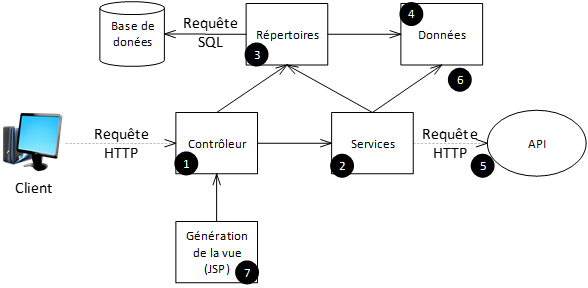
\includegraphics[width=10cm]{../img/part3/archi_actuelle_front.png}
				\caption{\label{archi_actuelle_front} Architecture simplifiée du Frontal
				de TrackCIS. Les flèche pleine représentent les dépendances entre les
				éléments.}
			\end{figure}
			
		\subsection{L'API permet de communiquer avec Cloverleaf}
			\paragraph{}% Les grandes lignes de l'archi de l'API
			L'API est développée avec la plateforme standard de Java ou Java SE (Standard
			edition) qui n'est pas destinée au développement web. En efet l'API n'est pas
			une application web, il s'agit d'un petit programme qui s'execute sur le même
			serveur que CLoverleaf et qui permet d'intéragir avec lui. L'API est
			cependant capable de reçevoir et d'interpréter des requêtes HTTP. Ceci est
			rendu possible grâce à la technologie Vertx. Il s'agit d'un ensemble de
			bibliothèque permettant mettant à disposition des développeurs des outils
			pour gérer la réception de requêtes HTTP.
			
			\paragraph{}
			On retrouve dans l'API des éléments similaire à ceux du Frontal. Tout d'abord
			un classe jouant le rôle de contrôleur permet de récupérer la reqûete HTTP
			envoyée par le Frontal et d'envoyer une réponse (figure
			\ref{archi_actuelle_api}, (1))). La réponse contient toutes les données
			demandées par le requête, pour la construire le contrôleur fait appel à des
			classes de services (2). Celles-ci vont se connecter à Cloverleaf et
			récupérer les informations demandées dans certaines bases de données de l'EAI. Les
			classes de services vont ensuite créer des classes de données (3) qui vont
			permettre au contrôleur de construir la réponse.
			\begin{figure}[H]
				\centering
				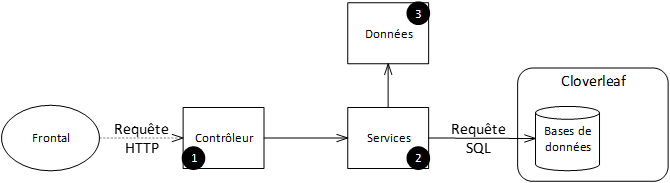
\includegraphics[width=9cm]{../img/part3/archi_actuelle_api.png}
				\caption{\label{archi_actuelle_api} Architecture simplifiée de l'API de
				TrackCIS.}
			\end{figure}
	
	\section{L'analyse technique permet d'implémenter le nouveau module sur
	l'existant}
		\paragraph{}
		A présent que nous savons comment est construit TrackCIS, nous pouvons
		commencer la conception du module statistique. Cette phase précède le
		développement à proprement parler. Son but est de cherches à définir tous les
		éléments techniques qui composerons le module, à savoir :
		\begin{itemize}
		  \item L'architecture, autrement dit la manière dont le code est structuré
		  \item Les outils utilisés, les bibliothèques, frameworks\ldots
		  \item Le modèle de données, c'est-à-dire la stcuture de la base de données
		\end{itemize}
		La contrainte est de nous adapter à l'architecture existante. Nous souhaitons
		y <<greffer>> le module statistique sans changer ce qui a déjà été mis en
		place que ce soit au niveau de l'API, du Frontal ou de la base de données.
		
		\subsection{Un module qui est basé sur les données disponibles dans
		Cloverleaf}
			\paragraph{}
			Les statistiques qui nous intéressent sont des données sauvegardées par l'EAI
			dans des base de données. LEs statistiques sont sauvegardées automatiquement
			à intervalles réguliers.
		
		
		\subsection{Nouvelle architecture de l'application}
			\paragraph{}% Une archi dessinée à partir des contraintes fonctionnelles
			Le module statistique de TrackCIS doit~:
			\begin{itemize}% Liste des contraintes
			  \item être basé sur l'architectture déjà en place. Il n'est pas question
			  dans ce projet de faire de grosses modifications sur l'existant. Ceci est
			  valable aussi bien pour le code lui-même que pour la structure de la base
			  de donnée.
			  \item être fermé à la modification et ouvert à l'extention. C'est-à-dire
			  qu'il doit être possible, pour une équipe de développement ultérieur,
			  d'ajouter des fonctionnalités au module sans ajour à modifier le code
			  existant.
			  \item ne pas perturber le fonctionnement de Cloverleaf. Pour afficher des
			  données pertinentes pour l'utilisateur, certains traitements seront
			  nécessaires sur les données brutes. Ceux-ci peuvent cependant ralentir ou
			  perturber le fonctionnement de Cloverleaf. Il est nécessaire pour cela que
			  ces traitements ne soient pas fait sur le serveur de l'EAI, donc pas au
			  niveau de l'API.
			  \item ne pas surchager le serveur sur lequel est déployé le frontal. Le
			  serveur servant à héberger le frontal n'est pas forcément une machine très
			  puissante, bien que cela varie en fonction des établissements.
			\end{itemize}
			
			\begin{figure}[H]
				\centering
				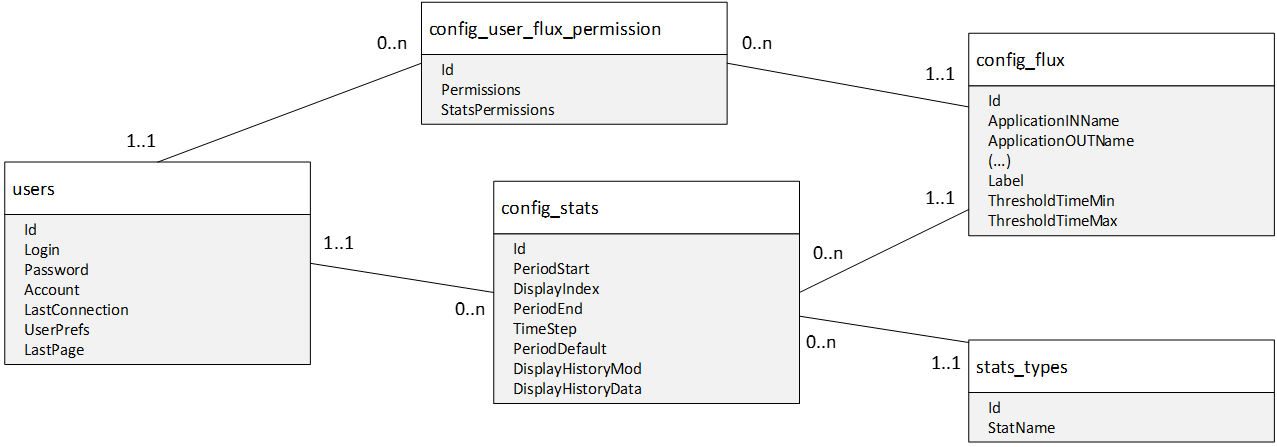
\includegraphics[width=16cm]{../img/part3/modele_donnee.png}
				\caption{\label{modele_donnee} Le nouveau modèle de donnée de TrackCIS au
				niveau du frontal.}
			\end{figure}
			
		\subsection{Réalisation des choix techniques}
			\paragraph{}% Liste des choix
			Le développement de ce projet implique l'utilisation d'un certain nombre de
			technologies. Certaines d'entre elles n'ont pas été utilisée pour le
			développement de la première version de TrackCIS.
			Le tableau ci-dessous résume l'ensemble des technologies qui ont été
			utilisées pour le développement de TrackCIS jusqu'a présent (c'est-à-dire
			avant le présent travail).
			
			\paragraph{}% Méthodo des choix
			Nous n'allons pas ici détaillé tous les choix techniques qui ont été fait.
			Nous mettrons en avant dans cette partie la méthodologie avec laquelle ces
			différents choix tecnique on été effectué en l'illustrant d'un exemple, en
			l'occurence le choix de la bibliothèque graphique javascript. Comme nous
			l'avons vu dans l'architecture de nouveau module, les graphiques sont
			dessinés par le navigateur client. La navigateur reçois un ensemble de script
			javascript qu'il sait interpréter. Certains de ces scripts permettrons donc
			d'afficher les graphiques. Pour cela nous avons besoin d'une bibliothèque
			javascript, c'est-à-dire un ensemble de fonctions précrites. Il en existe de
			très nombreuses et certaines sont gratuites et libres. Pour faire notre choix
			nous partons des contraintes suivantes~:
			\begin{itemize}
			  \item La bibliothèque doit être gratuite et son utilisation pour la
			  création de produits commerciaux doit l'être également.
			  \item Elle doit permettre à minima de dessiner les types de graphiques
			  spécifiés dans les fonctionnalités (courbe et historgamme avec plusieurs
			  séries de données, jauge et donut).
			\end{itemize}
			% Listing des librairies qui répondent à ces critères
			Nous retenons une liste de N bibliothèques qui respectent ces deux critères.
			Pour n'en retenir qu'une nous les comparons à l'aides d'autres critères qui
			sont~:
			\begin{itemize}
			  \item La qualité et la disponibilité de la documentation et de la
			  communauté d'utilisateur. Il est importatn de penser à la suite du projet
			  et aux améliorations future du module. Une bonne documentation nous
			  permettra d'aller plus vite dans l'implémentation et également à une équipe
			  de développement ultérieur de s'approprier plus facilement le code pour y
			  ajouter des graphique ou corriger des bugs.
			  \item L'estétisme et la possibilité de personalier les graphique. Certaines
			  bibliothèque propose des graphiques prêts à l'emplois, ce qui présente un
			  gain de temps certain pour le développement. Cependant, le module
			  statistique doit respecter la charte graphique déjà en place dans l'outil.
			  \item La possibilité de faire de petites animations de transition. Cela
			  peut être par exemple un petit effet à l'appartion d'une courbe, ou la
			  possibilité d'afficher une infobulle lors du passage de la sourie sur un
			  point de donnée du graphique.
			  \item La possibilité de pouvoir dessiner d'autres types de graphique. Nous
			  ne pouvons pas prévoir comment évolura le module ni quelles nouvelles
			  données seront rendu accessibles par Cloverleaf dans le future. Nous devons
			  choisir une bibliothèque nous laissant suffisament de possibilité pour
			  pouvoir représenter d'autres types de graphiques.
			\end{itemize}
			Tous ces critères ne sont pas égaux, certain sont plus important que
			d'autres. C'est pourquoi nous allons les pondérer à l'aide d'une note sur
			dix. Nous notons ensuite les six bibliothèques retenue sur chacun de ces
			critère, puis nous appliquons la pondération à chaque note. La note globale
			de chaque bibliothèque est le total des notes podérées de chque critère. Le
			tableau \ref{choix_bib_js} présente le résultat de cette méthode.
			\begin{table}[H]
				\centering
				\caption{\label{choix_bib_js} Choix de la bibliothèque graphique
				javascript : d3js se démarque des autres.}
				\begin{tabular}{| p{2cm} | p{2cm} | p{2cm} | p{2cm} | p{2cm} |
				p{2cm} | p{2cm} |}
					\hline
						\thead{Bibliothèque}
						&\thead{Documentation}
						&\thead{Simplicité d'utilisation}
						&\thead{Esthétisme}
						&\thead{Annimations}
						&\thead{Autres graphiques possibles}
						&\thead{Total}
						\\
					\hline
						D3&10&1&10&10&10&\thead{244}
						\\
					\hline
						Google Charts&10&9&5&5&9&\thead{230}
						\\
					\hline
						Chartist&8&6&8&10&5&\thead{202}
						\\
					\hline
						EJS Chart&7&8&7&2&8&\thead{196}
						\\
					\hline
						JQPlot&6&8&6&5&8&\thead{186}
						\\
					\hline
						RGraph&6&9&2&4&5&\thead{146}
						\\
					\hline
				\end{tabular}
			\end{table}
			La bibliothèque retenue est D3 (Data driven document), 
			open source et gratuite permettant de construire n'importe quel type de
			visualisation de données.
			
	\section{Une gestion de projet en mode agile}
		\paragraph{}
		La phase de conception est maintenant terminée et les choix technique
		réalisés. Nous pouvons à présent passer à l'implémentation à proprement
		parler, c'est à dire à la production du code.
		
		\subsection{Une méthodologie qui s'inspire des méthodes agiles}
			\paragraph{}% C'est quoi l'agilité et pourquoi ce choix
			Pour cette dernière étape nous nous insprirons des méthodes agile, nottement
			de la méthode Scrum. La méthode Scrum est basée sur des ittérations
			succèssives, les Sprint. A chaque ittération, un petit morceau d'application
			est présenté au commanditaire, dans notre cas Xperis. Ceci permet d'obtenir
			un produit final qui colle au plus près des attentes du commanditaire puisque
			celui-ci devient un acteur à part entière du projet. A chaque ittération il
			peut en effet donner son avi sur ce qui a été développé et demander des
			améliorations ou changer ce qui avait été initaliement prévu pour le sprint
			suivant.
			
			\paragraph{}% Le backlog et les US
			Le développement d'une application en sprints implique d'être en mesure de
			produire quelque chose de présentable à l'issue du sprint, donc de visuel.
			Cela implique également de ségmenter l'application en petites parties que
			l'on pourra développée indépendament les unes des autres : les user stories.
			Une user story correspond à une petite histoire d'utilisation de
			l'application, c'est un petit morceau de l'epérience de l'utilisateur. Voici
			quelques exemples d'user stories :
			\begin{itemize}
			  \item 
			\end{itemize}
			
			\paragraph{}% Les sprints
			Nous chaoisirons des sprint d'une durée de deux semaine. Un sprint se déroule
			en suivant les étapes suivantes :
			\begin{itemize}
			  \item[1) ] 
			\end{itemize}
			
			
			\begin{figure}[H]% Méthodo du développement
				\centering
				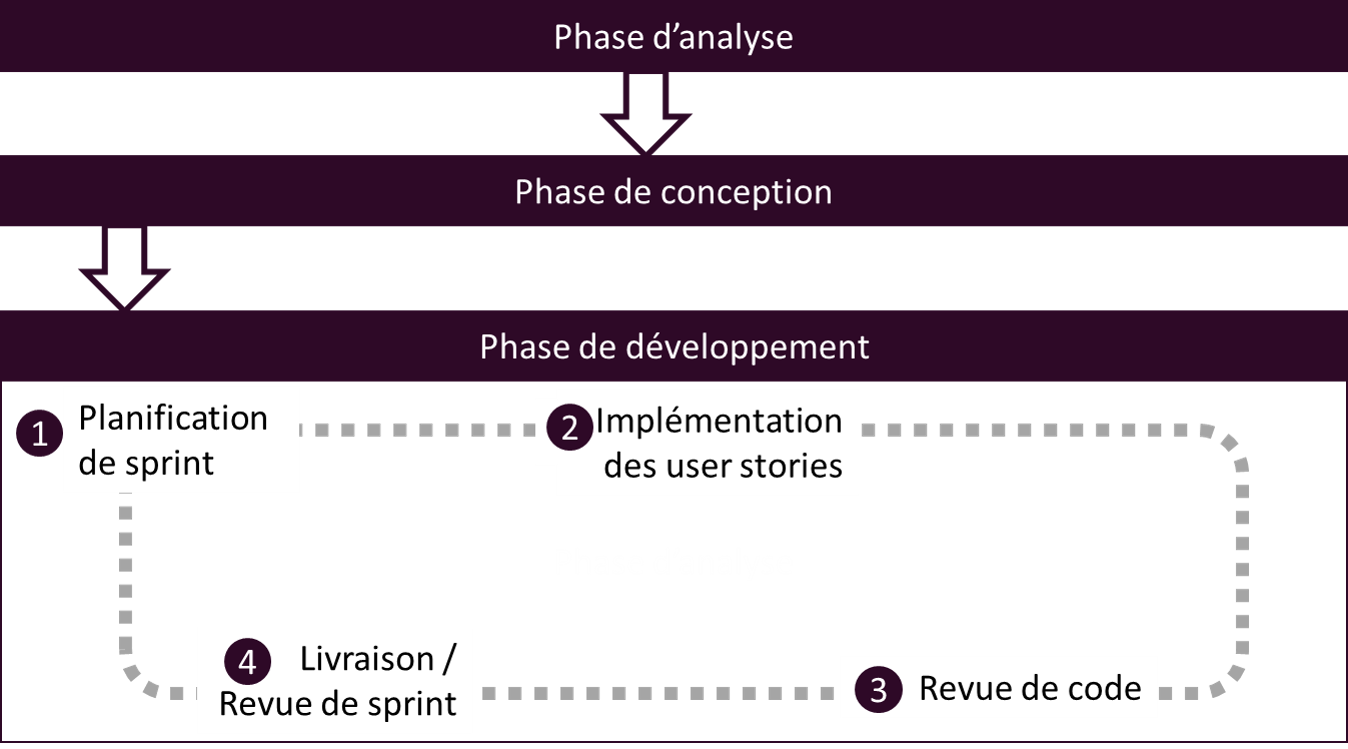
\includegraphics[width=15cm]{../img/part3/methodo_dev.png}
				\caption{\label{methodo_dev} Le développement se déroule en sprints de
				deux semaines chacun.}
			\end{figure}
		
		\subsection{Élaboration du backlog}
			\paragraph{}% Passage des fonctionnalités aux user stories
			
			
			Pour construire notre backlog, nous devont établir une liste de user sotries.
			De la même manière que nous avons établi un lien entre besoins et
			fonctionnalités, il est possible de relier ces dernières aux user stories.
			Une fonctionnalité peut être découpée en plusieurs user stories, comme le
			montre la figure \ref{mapping_fonctios_us}, une user story n'est liée qu'à
			une seule fonctionnalité.
			\begin{figure}[H]% Mapping fonctionnalités -> US
				\centering
				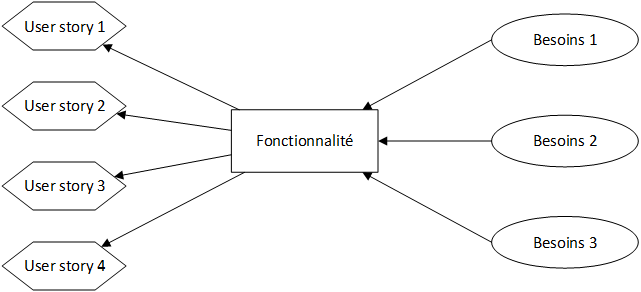
\includegraphics[width=7cm]{../img/part3/mapping_fonctios_us.png}
				\caption{\label{mapping_fonctios_us} Chaque fonctionnalité est redécoupée
				en une ou plusieurs user stories.}
			\end{figure}
			
			\paragraph{}% Priorisations des US
			Le backlog est la base de travail pour le développement. C'est à la fois
			unoutil de spécification décrivant finement les fonctionnalités du module, et
			un outil de gestion de projet car il permet de suivre son avancement. Le
			backlog permet également de planifier le travail. Pour cela il faut en
			prioriser les élements.\newline
			
			
			Pour estimer la difficulté intrinsèque au développement de chaque user story,
			nous emploirons la technique dite du planing poker. Nous utiliserons comme
			base les premiers éléments de la suite de Fibonacci (1, 2, 3, 5, 8, 13, 21,
			34,\ldots). Nous attriburons une note médianne à une storie que nous
			évaluerons de difficulté moyenne. En l'occurence % TODO
			
			Puis nous noterons les autres stories à relativement à la première en
			n'utilisant que des éléments de la suite de Fibonacci.
			
	
	\section{Bilan de la phase de développement et suite du projet}
		\paragraph{}
		Cette dernière partie est l'occasion de faire le bilan sur ce qui a été
		implémenté.
		
		\subsection{Les fonctionnalités implémentées}
			\paragraph{}% Bilan quantitatif de ce qui a été fait et reste à faire
		
			\paragraph{Historique de nombre de messages par flux~: }
			
			\paragraph{Valeur moyenne du temps de transfert d'un message dans le flux~: }
		
		\subsection{Les limites du projet}
			\paragraph{}% présentation
			Tout au long de ce prjet nous avons été amené à faire un certain nombre de
			choix, parfois de manière très arbitraire. Revenous ici sur les principales
			limites de la méthodologie globale du projet visant à améliorer TrackCIS et
			voyons comment nous pouvons en tirer les leçons pour préparer la suite du
			projet.
		
			\paragraph{}% Le choix de développer le module statistique est arbitraire
			
			\paragraph{}% La priorisation (besoins, fonctios et US) sont aussi
			% arbitraires
			
		\subsection{Les suites possibles du projet pour Xperis}
			\paragraph{}% Les gros modules a développer à partir de l'ADB
			
			\paragraph{}% Les <<petites>> amélioration à faires
			
			